\documentclass{article}

% Language setting
% Replace `english' with e.g. `spanish' to change the document language
\usepackage[english]{babel}
\usepackage{caption}
% Set page size and margins
% Replace `letterpaper' with`a4paper' for UK/EU standard size
\usepackage[letterpaper,top=2cm,bottom=2cm,left=3cm,right=3cm,marginparwidth=1.75cm]{geometry}

% Useful packages
\usepackage{amsmath}
\usepackage{graphicx}
\usepackage{authblk} % this is for multiple autho  rs 
\usepackage[colorlinks=true, allcolors=black]{hyperref}
\usepackage{cleveref}
\usepackage{booktabs}
\usepackage{multirow}
\usepackage{threeparttable} % For footnotes in tables
\usepackage{graphicx}  % For including graphics
\usepackage{caption}   % For customizing captions
\usepackage{cleveref}  % For enhanced referencing

% Configure for "Fig.":
\crefname{figure}{figure}{figures}
\Crefname{figure}{Figure}{Figures}


% reference configuration
\usepackage[authoryear,round]{natbib}
\bibliographystyle{apalike} % for an APA-like style
\usepackage{amsmath}

% reference configuration
\usepackage[authoryear,round]{natbib}
\bibliographystyle{apalike} % for an APA-like style

%%%%%%%%%%%%%%%%%%%%%%%%%%%%%%%%%%%%
%%% --- Tittle of the paper --- %%%
%%%%%%%%%%%%%%%%%%%%%%%%%%%%%%%%%%
\title{\textbf{Supplementary materials: Development of outdoor air pollution models for estimating exposure in the Barcelona Life Study Cohort (BiSC)}}

%%%%%%%%%%%%%%%%%%%%%%%%%%%%%%%%%%%%%%%%%
%%% --- Authors and affiliations --- %%%
%%%%%%%%%%%%%%%%%%%%%%%%%%%%%%%%%%%%%%%

%%% --- Authors --- %%%
\author{Alan Domínguez, Payam Dadvand, Marta Cirach, Bruno Raimbault, Toni Galmes, Karl Samuelsson, Mark Nieuwenhuijsen, Jordi Sunyer, Xavier Basagaña, Ioar Rivas}
%%%%%%%%%%%%%%%%%%%%%%%%%%%%%%%%%%%%%%%%%%%%%%%%%%%%%%%%%%%%%%%%%%%%%%%%%

\begin{document}
\maketitle

%%%%%%%%%%%%%%%%%%%%%%%%%%%%%%%%%%%%%%%%%%%%%%
%%% --- Land Use Regression modelling --- %%% 
%%%%%%%%%%%%%%%%%%%%%%%%%%%%%%%%%%%%%%%%%%%%
\section{Land Use Regression modelling details}

%%%%%%%%%%%%%%%%%%%%%%%%%%%%%%%%%%%%%%%%%%%%%%%%%%%%%%%%%%%%%%%
%%% --- Predictor variables and sources of information --- %%% 
%%%%%%%%%%%%%%%%%%%%%%%%%%%%%%%%%%%%%%%%%%%%%%%%%%%%%%%%%%%%%%
\subsection{Predictor variables and sources of information}
To develop LUR models, we calculate a set of spatial variables that could hep us to explain pollutant concentration distribution across the study area. We calculate a total of 101 predictor variables, see \textbf{\Cref{Table S1}}. To calculate the predictor variables we applied a wide range of local and regional GIS datasets, see \textbf{\Cref{Table S2}}. 

%%%% ----------------------------------------------------------------------------------%%%%
%%%% --- Table S1. Predictor variables categories created for LUR model development --- %%%
%%%% ----------------------------------------------------------------------------------%%%%

\renewcommand{\thetable}{S\arabic{table}}
\begin{table}[ht]
\centering
\caption{Predictor variables categories created for LUR model development.}
\begin{tabular}{lll}
\toprule
\textbf{Traffic} & \textbf{Land-uses} & \textbf{Urban configuration} \\
\midrule
Road length & Residential & Population \\
Major road length & Industry & Buildings density \\
Distance to road & Natural & Imperviousness \\
Distance to major road & Urban green & Slope \\
Traffic intensity & Road density & Buildings height \\
Traffic intensity only major roads &  & Street bearing \\
Traffic intensity in nearest road &  & Low Emission Zone (ZBE)\\
Traffic intensity in nearest major road &  & Street width (BiSCAPE)\\
                                         &  & Street canyon (BiSCAPE)\\
                                         &  & Sampler height (BiSCAPE)\\
\bottomrule
\label{Table S1}
\end{tabular}
\end{table}

\vspace{-2em}

%%%% ------------------------------------------------------%%%%
%%%% --- Table S2. Data sources for predictor variables --- %%%
%%%% ------------------------------------------------------%%%%
\begin{table}[ht]
\centering
\caption{Predictor varaibles categories created for LUR model development.}
\begin{tabular}{lll}
\toprule
\textbf{Predictor variable} & \textbf{Year} & \textbf{Source} \\
\midrule
Road network and traffic data  & 2014 & Departament de mobilitat, Ajuntament de Barcelona \\
Land uses & 2018 & Urban atlas, Copernicus \\
Population & 2016 & Institut d'Estadística de Catalunya \\
Buildings height & 2009 & Modelo Digital de Superficies Edificación  - MDSn2.5 (MDSNE)\\
Imperviousness & 2018 & Copernicus \\
Slope & 2012 & Institut Cartográfic de Catalunya \\
ZBE & 2012 & OSM\\
\bottomrule
\label{Table S2}
\end{tabular}
\end{table}


%%%%%%%%%%%%%%%%%%%%%%%%%%%%%%%%%%%%%%%%%%%%%%%%%%%
%%% --- Deseasonalizing air pollution data --- %%% 
%%%%%%%%%%%%%%%%%%%%%%%%%%%%%%%%%%%%%%%%%%%%%%%%%%
\newpage
\subsection{Deseasonalizing pollution data}

For the development of LUR models data collected at different points of time need to be deseasonalized (process explained below) before being averaged to represent the average value of the baseline period. 

\subsubsection{NO\textsubscript{2} deseasonalization}

For the NO\textsubscript{2} data (BiSCAPE + BiSC) the \textit{difference method} was used for deseasonalisation. 

\begin{enumerate}
    \item Define the baseline period, that is, the total period in which the air pollution measurements were done. For NO\textsubscript{2} the baseline period was from 23\textsuperscript{rd} October 2018 to 16\textsuperscript{th} February 2022.
    \item Collect hourly air pollution data from a routine monitoring site covering the baseline period. We used data from Palau Reial monitoring station, as this is the reference site for the BiSCAPE campaigns and the BiSC cohort. NO\textsubscript{2}, data at Palau Reial was missing for only 5 \% of the period. Even though the missing rate is low, we imputed missing data by doing a linear regression with NO\textsubscript{2} levels at the monitoring site of Sants (r = 0.84). After recovering those data, the percentage of missing data at Palau Reial decreased to 0.68 \%. 
    \item Calculate the average concentration of NO\textsubscript{2} for the routine monitoring site covering the baseline measurement period: C\textsubscript{PR}(avg).
    \item Calculate the concentrations of the pollutant at the routine monitoring site for the exact same period (t) as the sample collected at the BiSC and BiSCAPE locations in the different periods: CP\textsubscript{PR}(t). 
    \item Calculate for the routine monitoring site for each sample the difference between the concentration (C\textsubscript{PR}) and the average covering the baseline measurement period: D\_C\textsubscript{PR}(t) = C\textsubscript{PR}(t) - C\textsubscript{PR}(avg).
    \item Calculate for each sample at site i (C\textsubscript{i}(t)) the adjusted concentration (C\textsubscript{i, adj}(t)) by computing: C\textsubscript{i,adj}(t) = C\textsubscript{i}/D\_C\textsubscript{PR}(t).
\end{enumerate}

\subsubsection{PM\textsubscript{2.5}, BC, PM\textsubscript{2.5 - Fe}, PM\textsubscript{2.5 - Cu}, PM\textsubscript{2.5 - Zn} deseasonalization}

For the PM\textsubscript{2.5}, BC, PM\textsubscript{2.5 - Fe}, PM\textsubscript{2.5 - Cu}, PM\textsubscript{2.5 - Zn} the data available was obtained during the BiSCAPE campaigns. The \textit{ratio method} was used for deseasoanlisation. The method procedure is very similar to the difference method explained. The rationale for using a different method for these pollutants is that we aim to create LUR models for some PM\textsubscript{2.5} components. Since we do not have hourly data from the PM\textsubscript{2.5} components for the baseline period (data is only available as a daily average every four days), the deseasonalisation of these components needs to be done with total PM\textsubscript{2.5} conctrations. As the \textit{ratio method} is based on subtraction, this method cannot be applied to different pollutants than the reference. Samples collected within the BiSCAPE campaigns at Palau Reial showed lower concentrations than those collected online at Palau Reial. Using the ratio method in PM\textsubscript{2.5} concentrations may lead to over-subtracting.

\begin{enumerate}
  \item Define the baseline period, that is, the total period in which the air pollution measurements were done. For PM\textsubscript{2.5} and its chemical components and BC the baseline period is from 01/01/2021 to 16/02/2022. 
  \item Collect hourly air pollution data from a routine monitoring site covering the baseline period. We used data from Palau Reial monitoring site, as this is the reference site for the BiSC cohort. 
  \begin{enumerate}
      \item PM\textsubscript{2.5} data at Palau Reial was missing for 26.8\% of the period due instrument maintenance. We imputed missing data by doing a linear regression with collocated BC concentrations (r=0.57) as no other station in Barcelona had hourly data for PM\textsubscript{2.5} during this period. After recovering those data, the percentage of missing data at Palau Reial decreased to 1.0\%. 
      \item BC data at Palau Reial was missing for only 2.3\% of the period
  \end{enumerate}
 \item Calculate the average concentration of the corresponding pollutant (j) for the routine monitoring site covering the baseline measurement period: C\textsubscript{j,PR}(avg). For PM\textsubscript{2.5} components, in this step j corresponds to total PM\textsubscript{2.5} mass concentrations.
 \item Calculate the concentrations of the pollutant j at the routine monitoring site for the exact same period (t) as the sample collected at BiSCAPE locations in the different periods: C\textsubscript{j,PR}(t). For PM\textsubscript{2.5} components, in this step j corresponds to total PM\textsubscript{2.5} mass concentrations. 
 \item Calculate the routine monitoring site for each sample the ratio between the concentration of pollutant j (C\textsubscript{j, PR}(t)) and the average covering the baseline measurement period: R\_C\textsubscript{j,PR} = C\textsubscript{PR}(t) / C\textsubscript{PR}(avg). For PM\textsubscript{2.5} components, in this step j correspond to total PM\textsubscript{2.5} mass concentrations.
 \item Calculate for each sample at site i (C\textsubscript{i}(t)) the adjusted concentration of pollutant j (C\textsubscript{i,adj}(t)) by computing: C\textsubscript{j,i,adj}(t) = c\textsubscript{j,i}(t)/R\_C\textsubscript{j,PR}(t)
\end{enumerate}

\subsubsection{Averages for LUR model development}
Once the measurements done at different time points (t) and sites (i) for the different pollutants (j) were deseasonalised, we proceeded to calculate the average of the adjusted cocnentrations for each site i. Therefore, the average value obtained for each site was considered to be the average for the baseline period at site i. These averages were the input values for the development of the LUR model. 

%%%%%%%%%%%%%%%%%%%%%%%%%%%%%%%%%%%%
%%% --- Performance metrics --- %%% 
%%%%%%%%%%%%%%%%%%%%%%%%%%%%%%%%%%
\newpage
\subsection{Performance metrics}
The following metrics were used to evaluate the LUR model for all the air pollutants assessed. 

% --- R2 --- %
\begin{equation}
R^2 = \left( \frac{\sum (\hat{y}_i - \bar{y})^2}{\sum (y_i - \bar{y})^2} \right)
\end{equation}

% --- root mean squared error (RMSE) --- % 
\begin{equation}
\text{RMSE} = \sqrt{\frac{1}{n} \sum_{i=1}^{n} (y_i - \hat{y}_i)^2}
\end{equation}

% --- correlation coefficient (r) --- %
\begin{equation}
r = \frac{\sum (x_i - \bar{x})(y_i - \bar{y})}{\sqrt{\sum (x_i - \bar{x})^2 \sum (y_i - \bar{y})^2}}
\end{equation}
\vspace{0.5 cm}

%%%%%%%%%%%%%%%%%%%%%%%%%%%%%%%%%%
%%% --- Model development --- %%%
%%%%%%%%%%%%%%%%%%%%%%%%%%%%%%%%%
\subsection{Model development}

Following the ESCAPE guidelines 




%%%%%%%%%%%%%%%%%%%%%%%%%%%%%%%%%%
%%% --- Model performance --- %%%
%%%%%%%%%%%%%%%%%%%%%%%%%%%%%%%%%
\subsection{Model performance}
The performance of the final models obtained for NO\textsubscript{2}, PM\textsubscript{2.5}, BC and PM\textsubscript{2.5 - Fe}, PM\textsubscript{2.5 - Cu}, PM\textsubscript{2.5 - Zn} is described in \textbf{\Cref{Table S3}}.  


%%% --- Table with performance metrics for Hybrid models --- %%%
\begin{table}[ht]
\centering
\begin{threeparttable}
\caption{Performance metric for LUR models.}
\label{Table S3}
\begin{tabular}{llllll}
\toprule
\textbf{Pollutant} & \textbf{Year} & \textbf{N}  &  \textbf{R\textsuperscript{2}\textsubscript{10-CV}} & \textbf{RMSE\textsubscript{10-CV}} & \textbf{Predictor variables}\tnote{1} \\
\midrule
\multirow{2}{*}{NO\textsubscript{2}} & \multirow{2}{*}{2018-2021} & \multirow{2}{*}{489} & \multirow{2}{*}{0.62} & \multirow{2}{*}{4.03} & trafload25 + sqralt + majorroadlength50 + \\ 
 & & & & & roadlength25 + majorroadlength300 \\
\midrule
PM\textsubscript{2.5} & 2019 & 34 & 0.45 & 1.47 & hdres500 + trafnear + ZBE \\
\midrule
BC & 2019 & 30  & 0.83 & 0.18 & hdres50 + linesnear + pop300 + trafload + roads500 \\
\midrule
PM\textsubscript{2.5 - Fe} & 2019 & 34 & 0.89 & 0.03 & trafnear + lat + pop + ZBE  \\
\midrule
PM\textsubscript{2.5 - Cu} & 2019 & 31 & 0.87 & 0.72 & trafnear + roads1000 + ind1000 + pop25 \\
\midrule
PM\textsubscript{2.5 - Zn} & 2019 & 31  & 0.85 & 6.99 & ZBE + roads50 + ind1000 + build25  \\
\bottomrule
\end{tabular}
\begin{tablenotes}
\small
\item[1] Predictor variables (roadlength: total road length (m), majorroadlength: total major road length (m), trafload: total traffic intensity (veh/day), trafnear: traffic intensity at the nearest road (veh/day), linesnear: number traffic lines on nearest street, ZBE: Low Emissions Zone (Yes/No, ref value=No), hdres: high-density residential area (m2), roads: roads surface area (m2), ind: industry area (m2), pop: population density (inhabitants), build: building area (m2), lat: latitude (m), sqralt: squared root altitude (m)).
\end{tablenotes}
\end{threeparttable}
\end{table}

The best models were selected based on its better validation performance and on the availability of the sampling campaign that could better represent the study population. 

%%%%%%%%%%%%%%%%%%%%%%%%%%%%%%%%%%%%%%%%%%%%%
%%% --- Back-extrapolation procedure --- %%%
%%%%%%%%%%%%%%%%%%%%%%%%%%%%%%%%%%%%%%%%%%%
\newpage
\subsection{Back-extrapolation procedure}

In the BiSC cohort study, we aim to study the effect of air pollution exposure using different windows of exposure (i.e., entire pregnancy, trimesters, and weeks of pregnancy). For each subject, back-extrapolated concentrations for different time periods can be calculated using daily concentrations from the background monitoring station. The station used was Palau Reial, the spatial location and the daily temporal concentration variability are shown for \textit{NO\textsubscript{2}}, \textit{PM\textsubscript{2.5}}, \textit{BC} in \textbf{\Cref{FigureS1}}.

%%% --- Figure. Monitoring stations and time-series used for LUR Back-Exptrapolation --- %%%

% Redefine the figure numbering to include 'S' for Supplementary
\renewcommand{\thefigure}{S\arabic{figure}}

%%% Figure: Monitoring stations and time-series used for LUR Back-Extrapolation %%%
\captionsetup[figure]{skip=6pt} % Adjusting the space between the figure and its caption
\begin{figure}[!htb]
    \centering
    \includegraphics[width=1.0\textwidth]{figures/location_ts_stations.png} % Adjust the path to your image
    \caption{Spatial location and daily temporal concentrations at Palau Reial station.}
    \label{FigureS1} % Label for referencing
\end{figure}



\newpage
%%%%%%%%%%%%%%%%%%%%%%%%%%%%%%%%%%%%%
%%% --- Dispersion modelling --- %%% 
%%%%%%%%%%%%%%%%%%%%%%%%%%%%%%%%%%%%


\section{Dispersion modelling details}

\subsection{Predictor variables and sources of information}

\subsection{Performance metrics}

\subsection{Model performance}


\newpage
%%%%%%%%%%%%%%%%%%%%%%%%%%%%%%%%%
%%% --- Hybrid modelling --- %%%%%%%%%%%%%%%%%%%%%%%%%%%%%%%%%%%%%%%%%%%%%%
%%%%%%%%%%%%%%%%%%%%%%%%%%%%%%%

\section{Hybrid modelling details}

\subsection{Predictor variables and sources of information}

\subsubsection{Spatial variables}

%%% Figure: Monitoring stations and time-series used for LUR Back-Extrapolation %%%
\captionsetup[figure]{skip=6pt} % Adjusting the space between the figure and its caption
\begin{figure}[!htb]
    \centering
    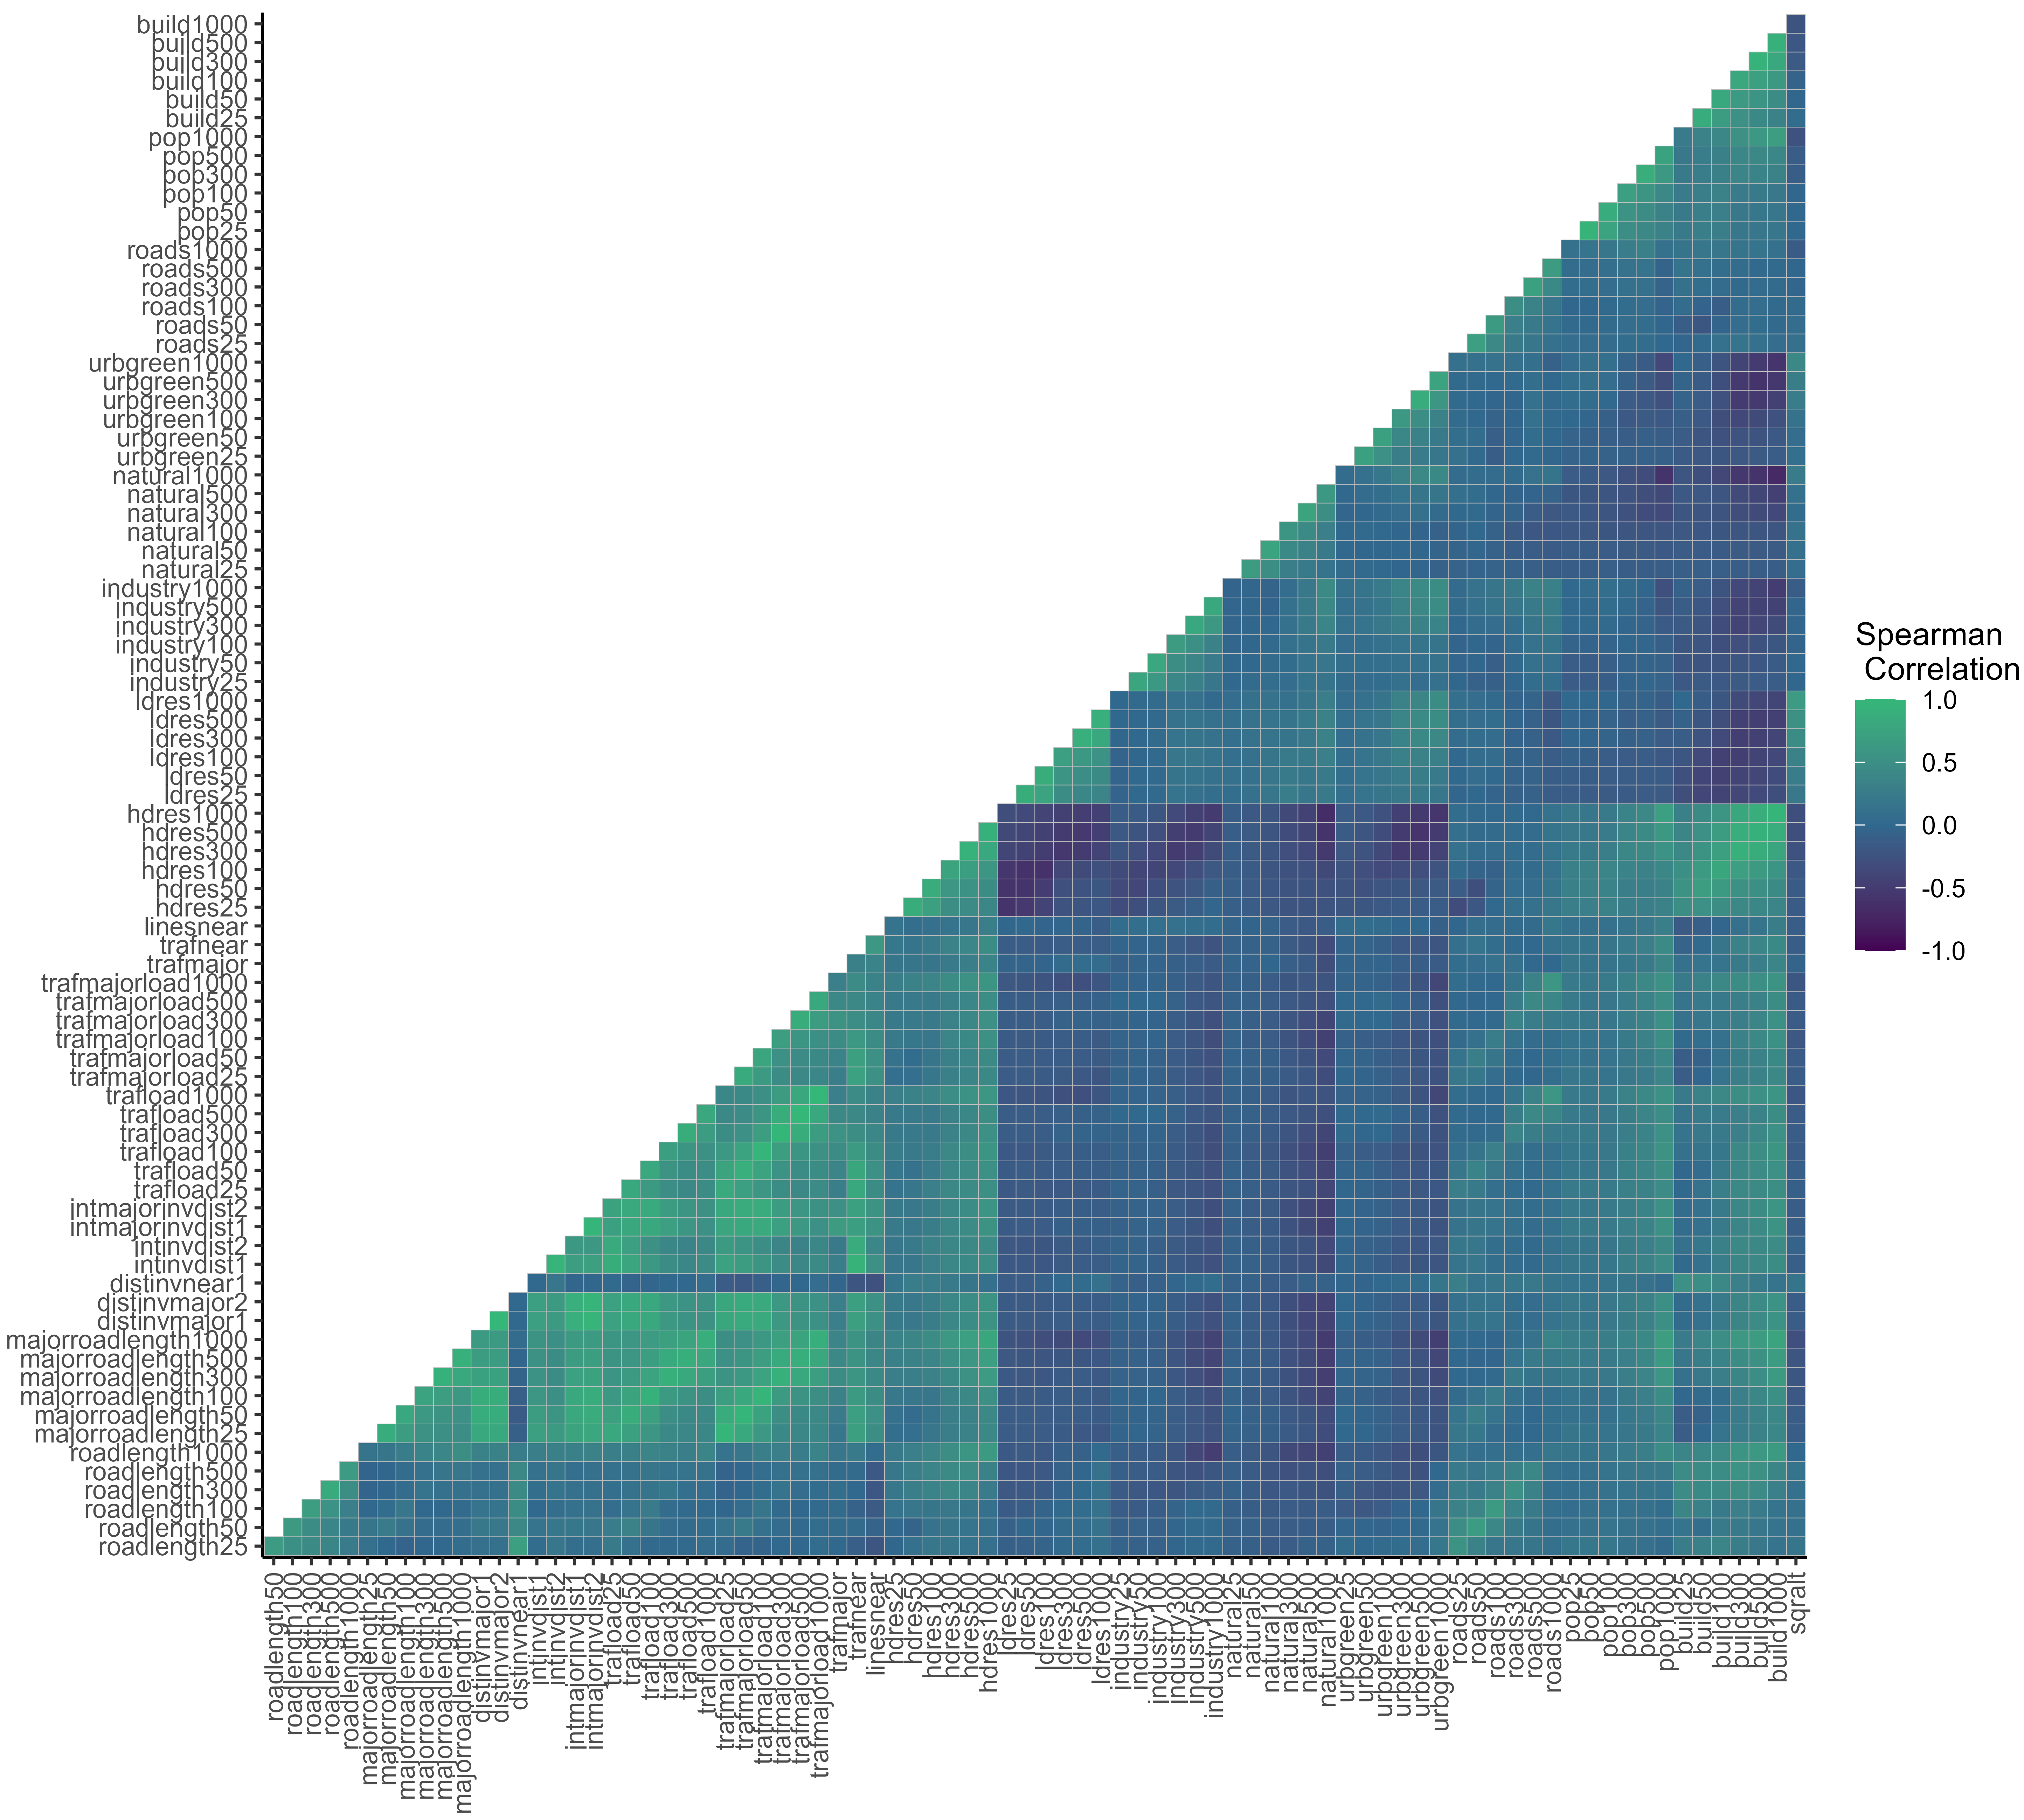
\includegraphics[width=0.6\textwidth]{figures/lur_pred_corr.png} % Adjust the path to your image
    \caption{Spatial location and daily temporal concentrations at Palau Reial station.}
    \label{FigureS1} % Label for referencing
\end{figure}


\subsubsection{Air pollution monitoring stations (XVPCA stations)}
%%% Figure: Monitoring stations and time-series used for LUR Back-Extrapolation %%%
\captionsetup[figure]{skip=6pt} % Adjusting the space between the figure and its caption
\begin{figure}[!htb]
    \centering
    \includegraphics[width=1.0\textwidth]{figures/location_ts_stations_hm.png} % Adjust the path to your image
    \caption{Spatial location and daily temporal concentrations at Palau Reial station.}
    \label{FigureS1} % Label for referencing
\end{figure}

\subsubsection{Traffic count measurement and meteorological data}
While our dispersion model initiall

\subsubsection{Dispersion model estimates}

\subsection{Performance metrics}
The following metrics were used to evaluate the HM for all the air pollutants assessed. 

% --- R2 --- %
\begin{equation}
R^2 = \left( \frac{\sum (\hat{y}_i - \bar{y})^2}{\sum (y_i - \bar{y})^2} \right)
\end{equation}

% --- root mean squared error (RMSE) --- % 
\begin{equation}
\text{RMSE} = \sqrt{\frac{1}{n} \sum_{i=1}^{n} (y_i - \hat{y}_i)^2}
\end{equation}

% --- correlation coefficient (r) --- %
\begin{equation}
r = \frac{\sum (x_i - \bar{x})(y_i - \bar{y})}{\sqrt{\sum (x_i - \bar{x})^2 \sum (y_i - \bar{y})^2}}
\end{equation}
\vspace{0.5 cm}

\clearpage
\begin{samepage}
\subsection{Model performance}
The performance metrics of the final HM for NO\textsubscript{2}, PM\textsubscript{2.5}, BC and PM\textsubscript{2.5 - Fe}, PM\textsubscript{2.5 - Cu}, PM\textsubscript{2.5 - Zn} is described in \textbf{\Cref{Table S4}}

%%% --- Table with performance metrics for Hybrid models --- %%%
\begin{table}[!htbp]
\caption{Performance metric for hybrid models.}
\label{Table S4}
\centering
\begin{threeparttable}
\small % Making the table text smaller
\begin{tabular}{llllll}
\toprule
\textbf{Pollutant} & \textbf{Year} & \textbf{N} & \textbf{R\textsuperscript{2}\textsubscript{10-CV}} & \textbf{RMSE\textsubscript{10-CV}} & \textbf{Predictors}\tnote{2} \\
\midrule
\multirow{6}{*}{NO\textsubscript{2}} & \multirow{6}{*}{2018-2021} & \multirow{6}{*}{1232} & \multirow{6}{*}{0.64} & \multirow{6}{*}{7.48} & no2\_dispersion +  idw\_no2\_monitoring\_station + \\
 & & & & & distinvmajor1 + majorroadlength100 + \\
 & & & & & majorroadlength50 + trafload25 + trafnear + \\ 
 & & & & & avg\_traffic\_stations + avg\_solar\_radiation + \\ 
 & & & & & sqralt + ldres1000 +ldres500 + hdres1000 + \\
 & & & & & build1000 + roads100 + lat + lon \\
\midrule
\multirow{5}{*}{PM\textsubscript{2.5}} & \multirow{5}{*}{2021} & \multirow{5}{*}{161} & \multirow{5}{*}{0.66} & \multirow{5}{*}{3.45} & pm25\_dispersion + idw\_pm25monitoring\_stations + \\
& & & & & avg\_traffic\_stations + ldres1000 + build25 + \\
& & & & & pop1000 + roads25 + sqralt  + \\
& & & & &  majorroadlength25 + trafload300 + \\
& & & & & build\_height\_25 + lat + lon \\
\midrule
\multirow{6}{*}{BC} & \multirow{6}{*}{2021} &\multirow{6}{*}{74} & \multirow{6}{*}{0.86} & \multirow{6}{*}{0.23} & bc\_dispersion + idw\_nox\_monitoring\_stations +\\ 
& & & & & avg\_atmospheric\_pressure + avg\_bc\_palau\_reial +   \\ 
& & & & &  pop100 + hdres300 + roads25 + avg\_wind\_speed +  \\
& & & & & roadlength25 + hdres50 + distinvmajor1 +  \\
& & & & & avg\_traffic\_stations + linesnear + \\
& & & & & pop300 + trafload500 + roads500 \\
\midrule
\multirow{4}{*}{PM\textsubscript{2.5 - Fe}} & \multirow{4}{*}{2021} & \multirow{4}{*}{161}  & \multirow{4}{*}{0.54} & \multirow{4}{*}{0.08} & pm25\_road\_nonexhaust + \\ 
& & & & & idw\_pm25\_monitoring\_stations + \\
& & & & & roads300 + roads1000 + ldres500 + \\
& & & & & sqralt + zbe + lat + lon \\
\midrule
\multirow{5}{*}{PM\textsubscript{2.5 - Cu}} & \multirow{5}{*}{2021} & \multirow{5}{*}{154} & \multirow{5}{*}{0.70} & \multirow{5}{*}{2.15} & pm25\_road\_nonexhaust + \\
& & & & & idw\_pm25\_monitoring\_stations + \\
& & & & & linesnear + industry1000 + roads300 + \\
& & & & & ldres1000 + roads1000 + avg\_traffic\_stations + \\
& & & & &  zbe + lat + lon \\
\midrule
\multirow{6}{*}{PM\textsubscript{2.5 - Zn}} &\multirow{6}{*}{2021} & \multirow{6}{*}{141} & \multirow{6}{*}{0.44} & \multirow{6}{*}{27.7} & pm25\_road\_nonexhaust + pm25\_background + \\
& & & & & idw\_pm25monitoring\_stations + linesnear + \\
& & & & & industry1000 + roads50 + build25 + roads300 + \\
& & & & & ldres1000 + roads1000 + avg\_traffic\_stations + \\
& & & & & trafmajor + trafmajorload1000 +  trafload1000 +\\
& & & & & hdres25 + zbe + lat + lon \\
\bottomrule
\end{tabular}
\begin{tablenotes}
\scriptsize
\item [2] Predictor variables (no2\_Dispersion: dispersion estimates (ug/m$^3$), pm25\_Dispersion: dispersion estimates PM2.5 (ug/m$^3$), BC\_Dispersion: dispersion estimates BC (ug/m$^3$), PM25\_road\_nonexhaust: dispersion estimates for nonexhaust PM2.5 (ug/m$^3$), PM25\_background: dispersion estimates for background PM2.5 (ug/m$^3$), idw\_no2\_monitoring\_station: weekly NO$_2$ inverse distance weighting interpolation estimates from XVCPA (ug/m$^3$), idw\_pm25\_monitoring\_station: weekly PM2.5 inverse distance weighting interpolation estimates from XVCPA (ug/m$^3$), idw\_nox\_monitoring\_station: weekly NOx inverse distance weighting interpolation estimates from XVCPA (ug/m$^3$), avg\_bc\_palau\_reial: weekly BC average concentration from Palau Reial monitoring station (ug/m$^3$), avg\_traffic\_stations: weekly average count of vehicles in AMB (count), avg\_solar\_radiation: weekly average solar radiation from Raval station (MJ/m$^2$), avg\_wind\_speed: weekly average wind speed from Raval station (km/h), avg\_atmospheric\_pressure: atmospheric pressure from Raval station (hPA), roadlength: total road length (m), majorroadlength: total major road length (m), trafload: total traffic intensity (veh/day), trafnear: traffic intensity at the nearest road (veh/day), linesnear: number traffic lines on nearest street, zbe: Low Emissions Zone (Yes/No, ref value=No), hdres: high-density residential area (m$^2$), roads: roads surface area (m$^2$), ind: industry area (m$^2$), pop: population density (inhabitants), build: building area (m$^2$), ldress: low density residential area (m$^2$), industry: industrial area (m$^2$), trafmajor: total major roads traffic intensity (veh/day), build\_height: averaged building height (meters), lat: latitude (m), sqralt: squared root altitude (m$^{1/2}$)).
\end{tablenotes}
\label{tablesX}
\end{threeparttable}
\end{table}
\end{samepage}
\clearpage



\newpage
\subsection{Variable importance Random Forest}

%%% --- Figure. Comparison between measurements and predictions values in the test dataset --- %%%
% Put the figure text closer to the Figure 3
\captionsetup[figure]{skip=6pt}
% We add the figure with the study domain 
\begin{figure}[!htb]
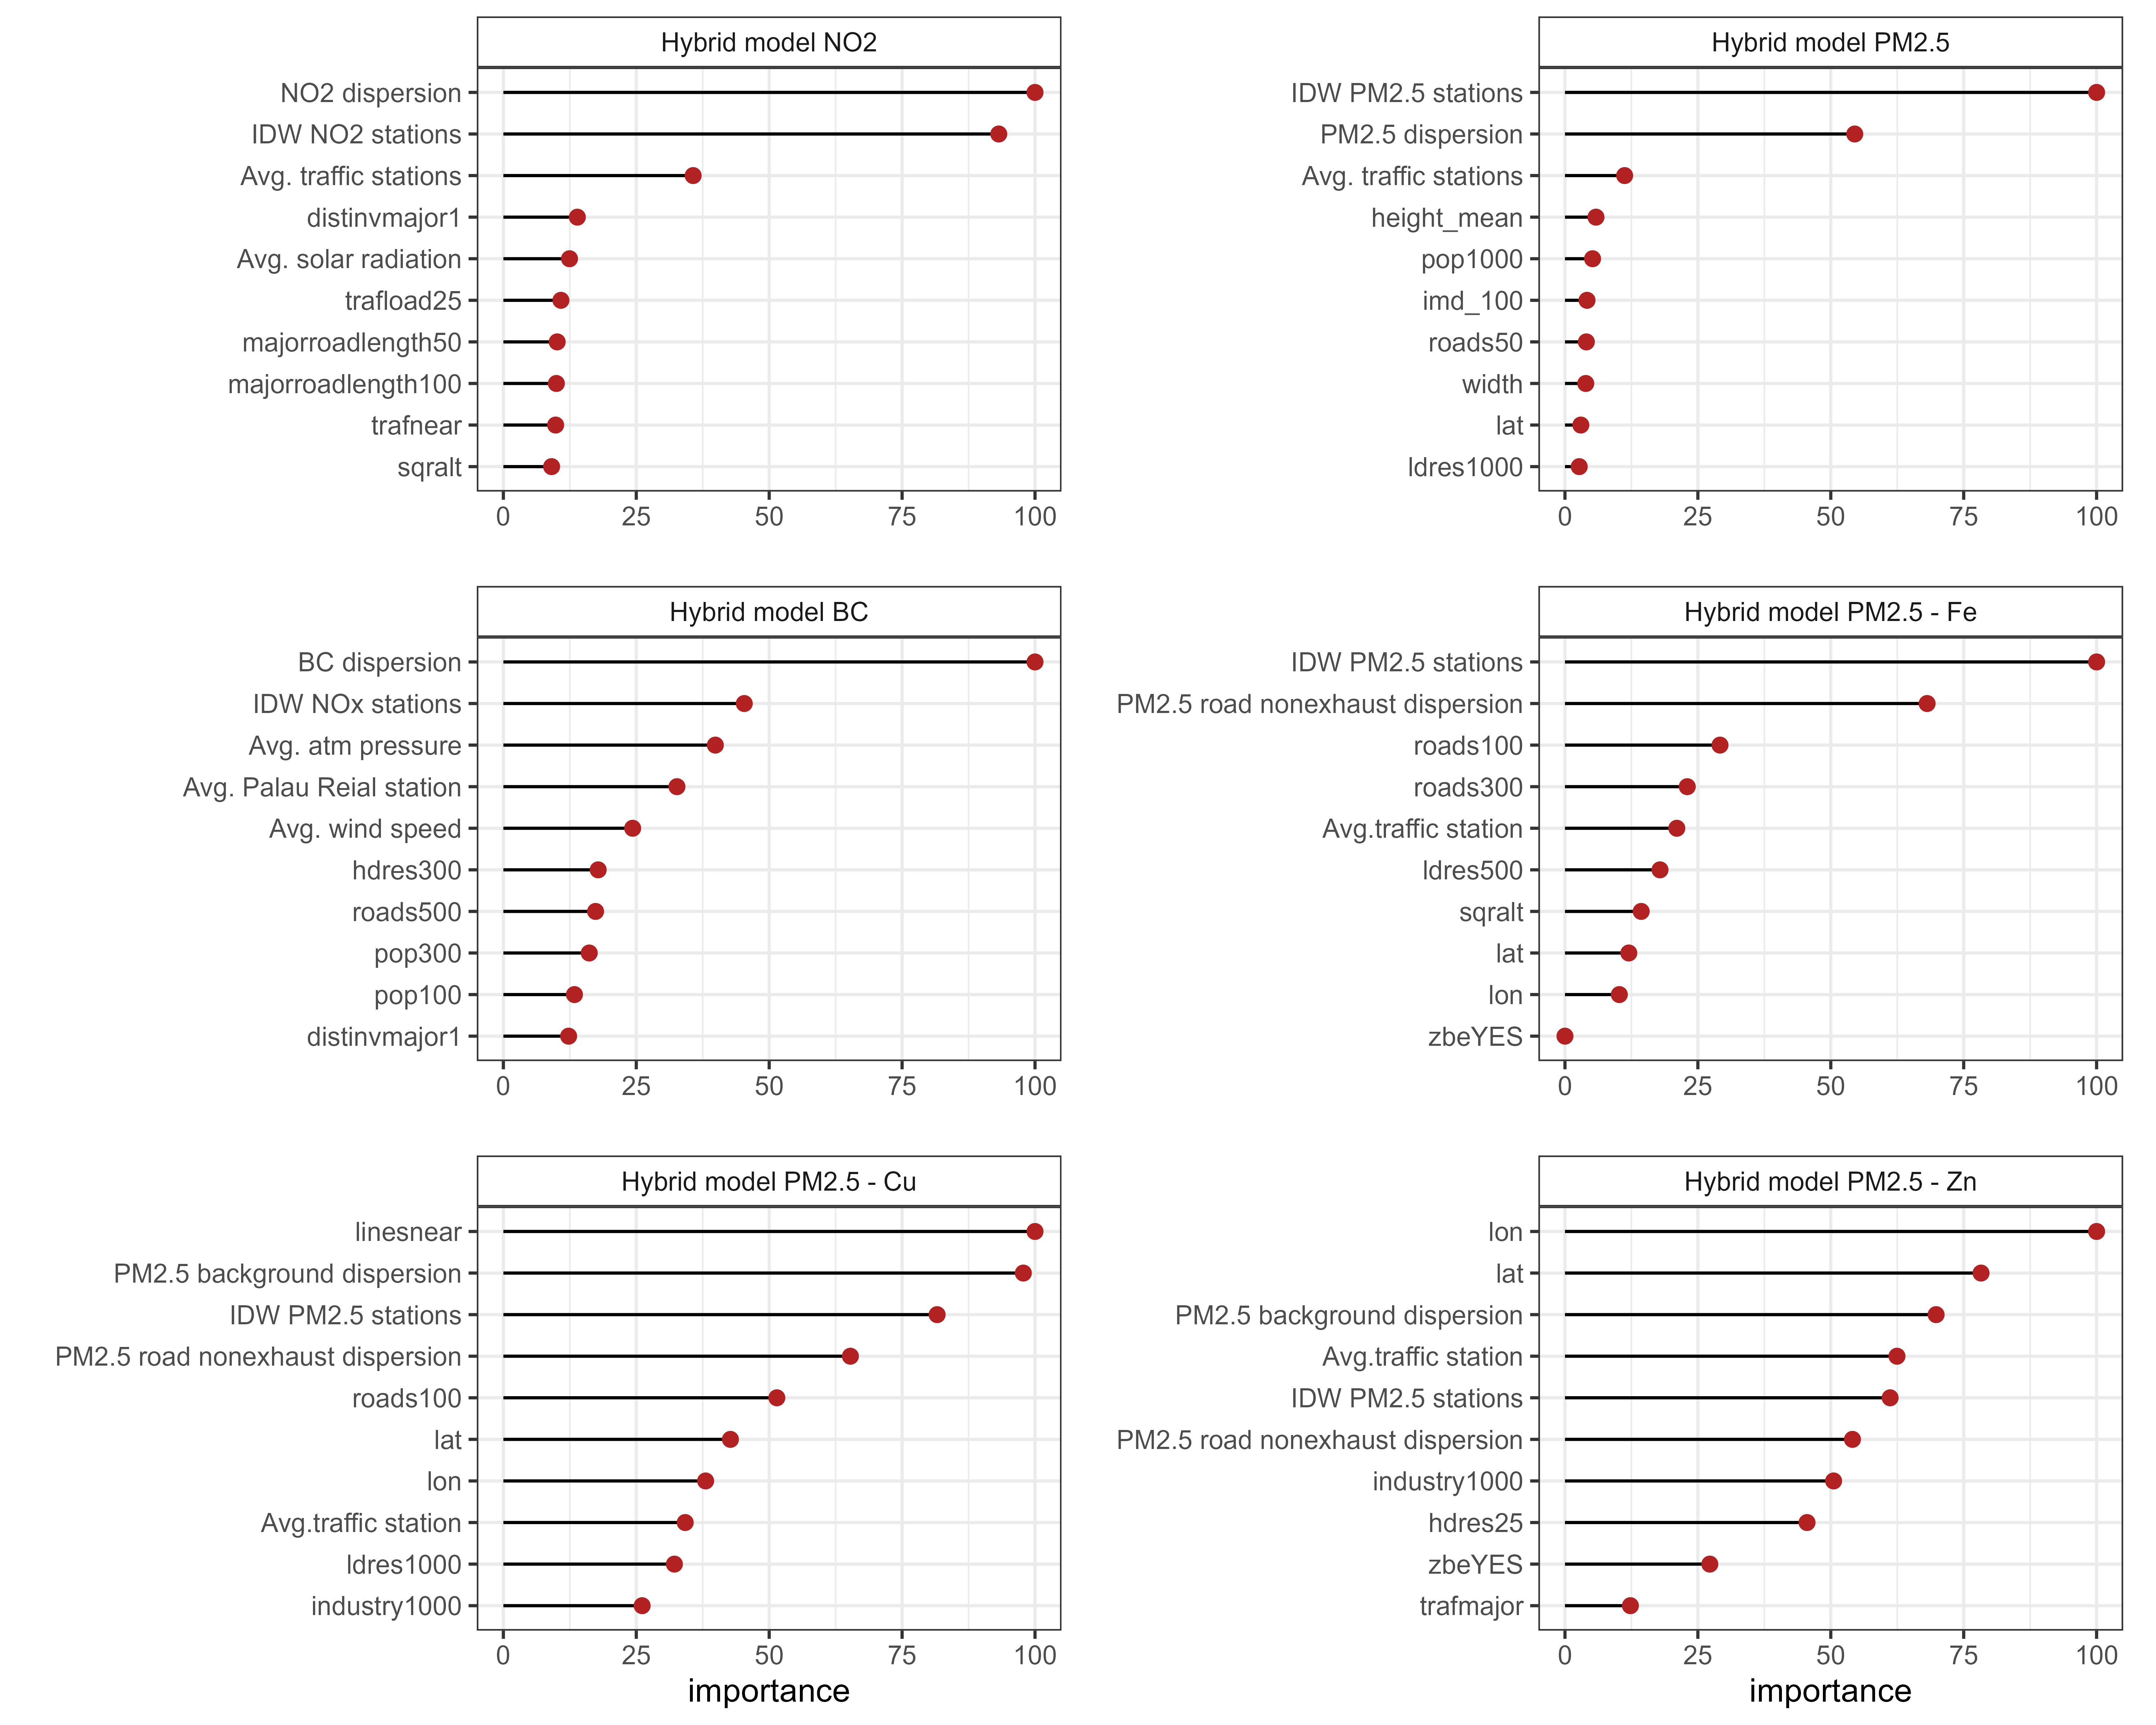
\includegraphics[width=1.0\textwidth]{figures/fig_HM_allmodels_importance_v2.png}
\caption{Variable importance for HM for \textit{NO\textsubscript{2}}, \textit{PM\textsubscript{2.5}}, \textit{BC}, \textit{PM\textsubscript{2.5 - Fe}}, \textit{PM\textsubscript{2.5 - Cu}} and \textit{PM\textsubscript{2.5 - Zn}.}}
\label{fig2}
\end{figure}

\newpage

\subsection{Comparison between observed measurements and predictions}

%%% --- Figure. Comparison between measurements and predictions values in the test dataset --- %%%
% Put the figure text closer to the Figure 3
\captionsetup[figure]{skip=6pt}
% We add the figure with the study domain 
\begin{figure}[!htb]
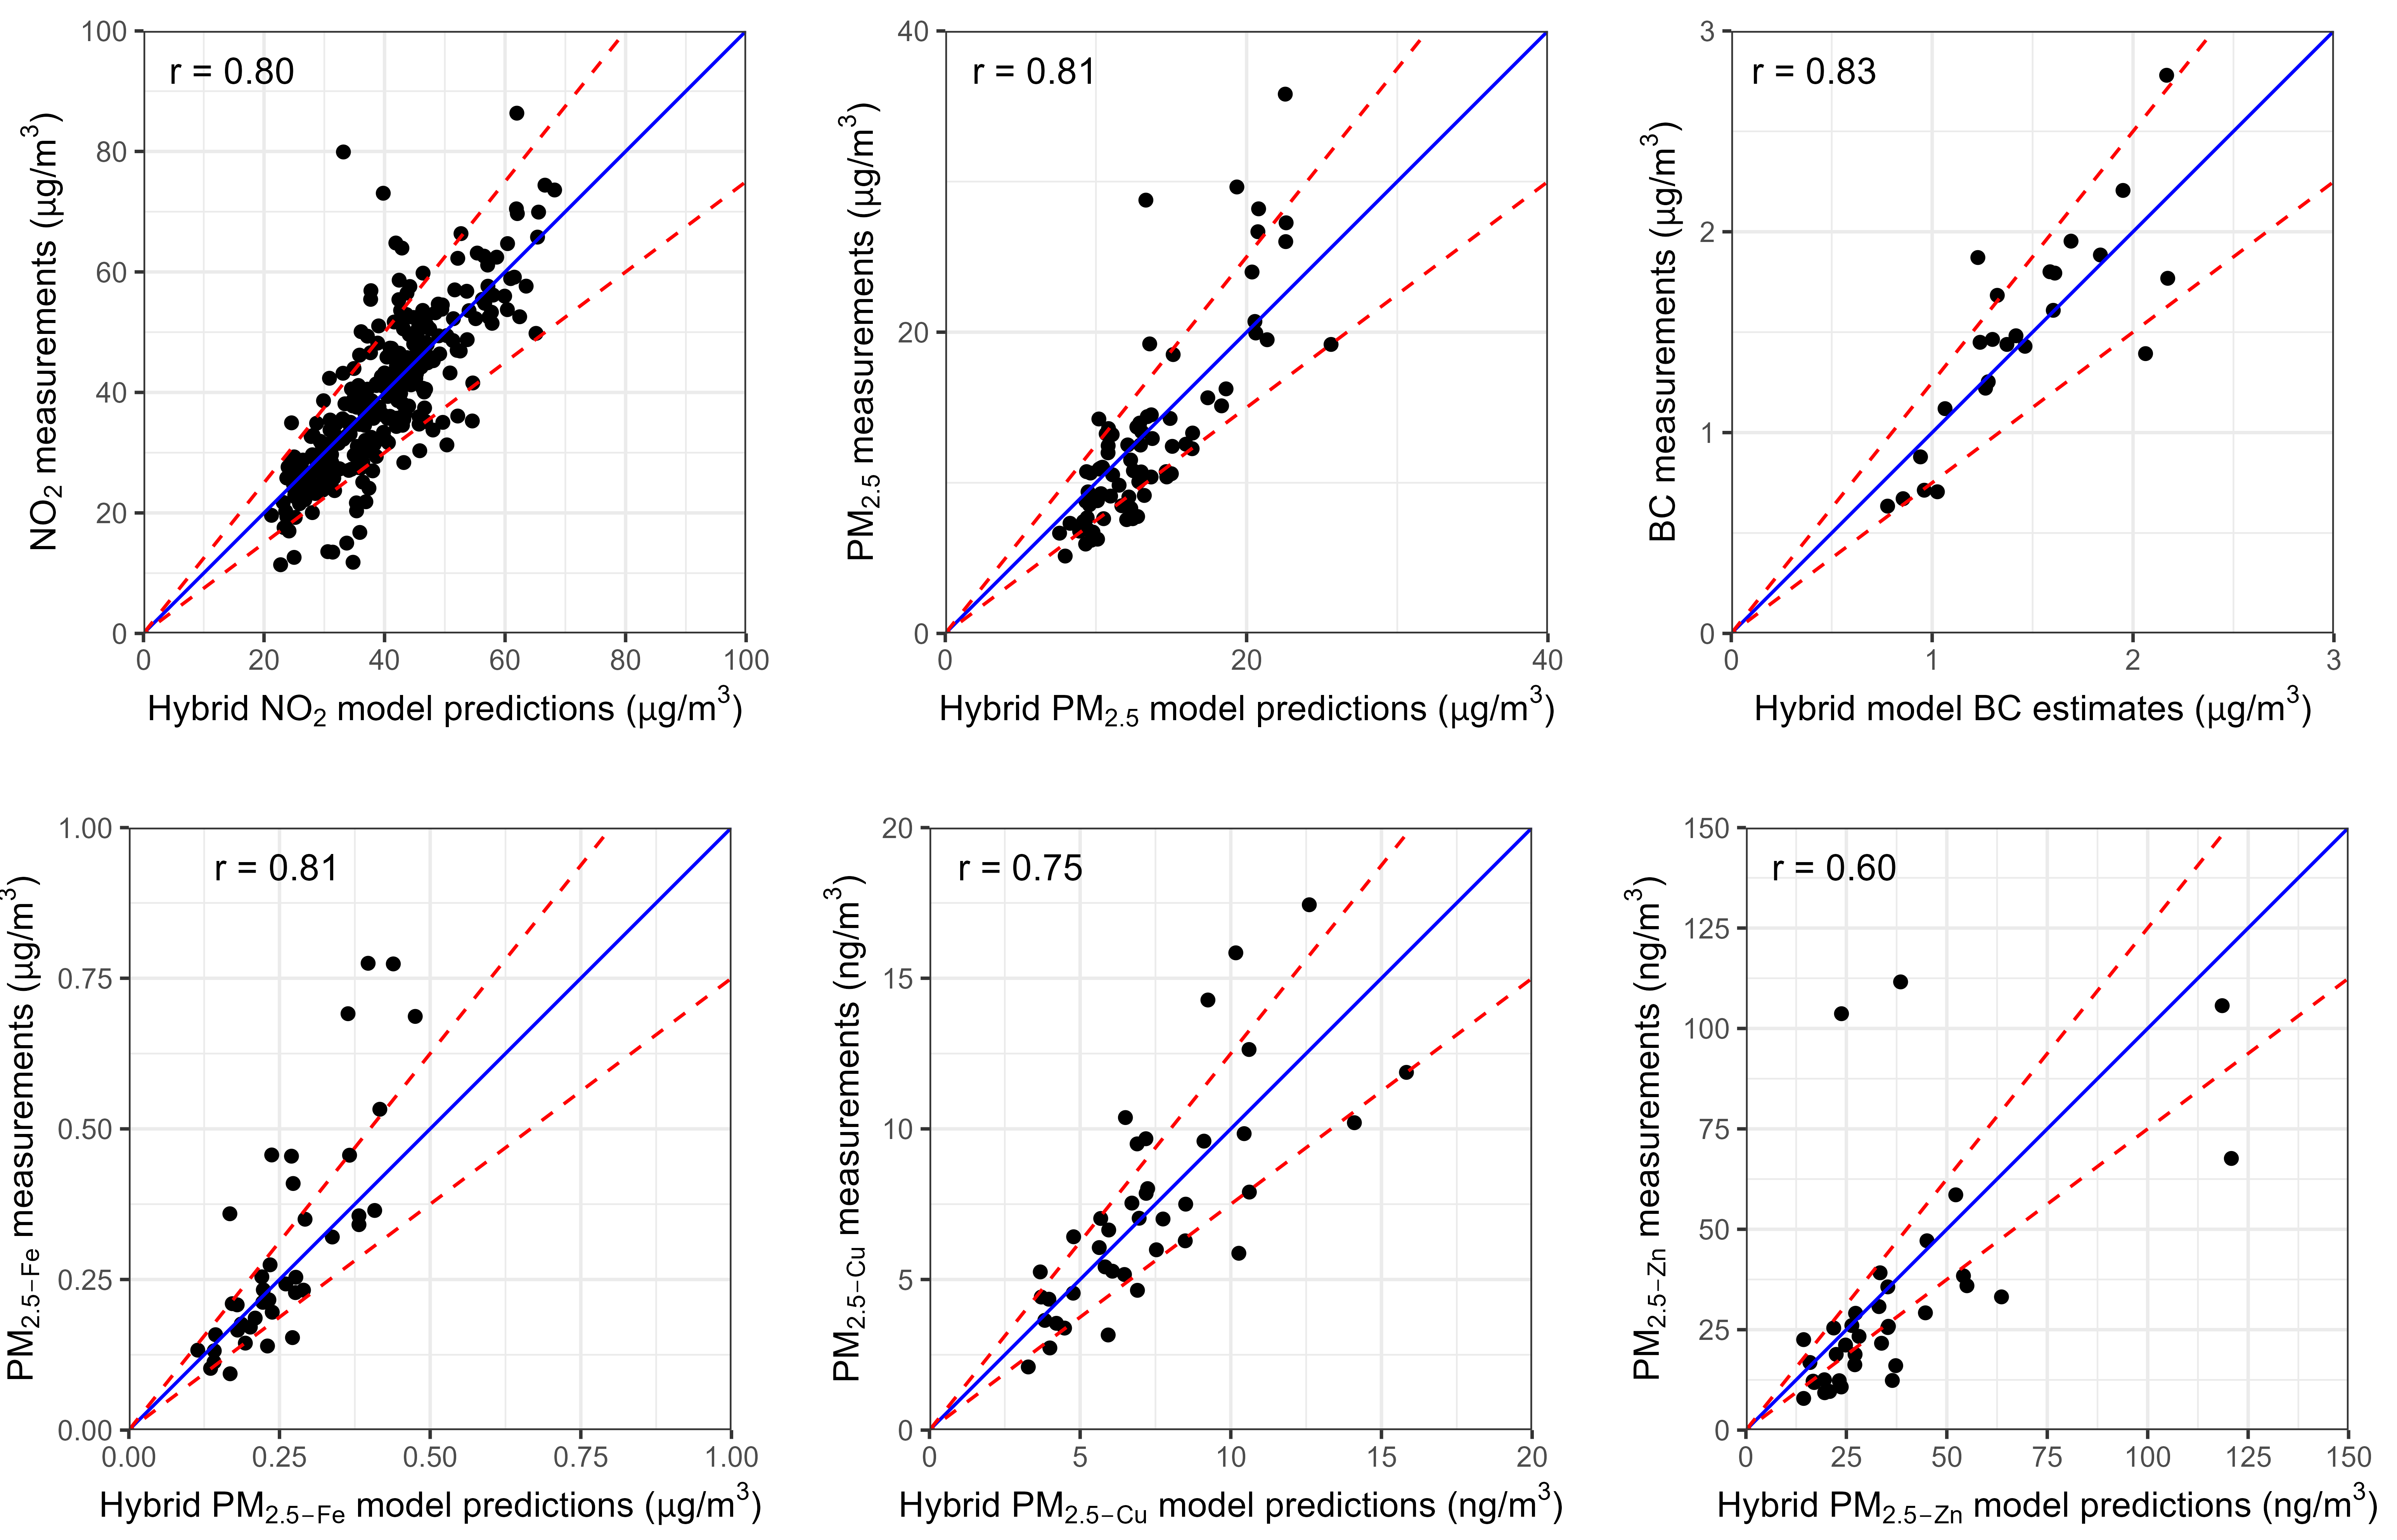
\includegraphics[width=1.0\textwidth]{figures/fig_HM_test_all_models_v2.png}
\caption{Comparison between measurements and prediction values for the hybrid models for \textit{NO$_2$}, \textit{PM$_{2.5}$}, \textit{BC}, \textit{PM\textsubscript{2.5 - Fe}}, \textit{PM\textsubscript{2.5 - Cu}}, and \textit{PM\textsubscript{2.5 - Zn}}.}
\label{fig2}
\end{figure}


%%%%%%%%%%%%%%%%%%%%%%%%%%%
%%% --- References --- %%%
%%%%%%%%%%%%%%%%%%%%%%%%%%%

\bibliography{references}


\end{document}